\section{Basic \Rev Commands}

\subsection{Introduction}

This tutorial demonstrates the very basic syntactical features of \RevBayes and \Rev. 
A more elaborate introduction into \Rev and probabilistic graphical models is provided .
A good reference for probabilistic graphical models for Bayesian phylogenetic inference is given in \cite{Hoehna2014b}.
The statistical examples are borrowed from a fourth year statistics course taught in the fall term 2011 at Stockholm University.

The first section of this tutorial involves 
\begin{enumerate}
\item Creating different types of variables.
\item Learning about functions. 
\end{enumerate}

Then we will see how to perform statistical inference using \RevBayes and \Rev  by implementing a Monte Carlo algorithm. 
Finally, we will see how \RevBayes 's built-in functions vastly simplify this inference task.

Let's start with the basic concepts for the interactive use of \RevBayes with \Rev (the language of \RevBayes). 
You should try to execute the statements step by step, look at the output and try to understand what and why things are happening. 
We start with some simple concepts to get familiar and used to \RevBayes. 
By now you should have executed \RevBayes and you should see the command prompt waiting for input. 
The best exercise is to write these statements exactly in \RevBayes. 

\subsection{Starting \RevBayes}
This tutorial demonstrates the basic syntactical features of \texttt{RevBayes} and the \texttt{Rev} scripting language.
Let's start with the basic concepts for the interactive use of \texttt{RevBayes} with \texttt{Rev} (the language of \texttt{RevBayes}). 
You should try to execute the statements step by step, look at the output and try to understand what and why things are happening.

First, open up your terminal and type \RevBayes.
This should launch \RevBayes and give you a command prompt (the \texttt{>} character).
This means \RevBayes is waiting for input.
\begin{figure}[H]
	\centering
	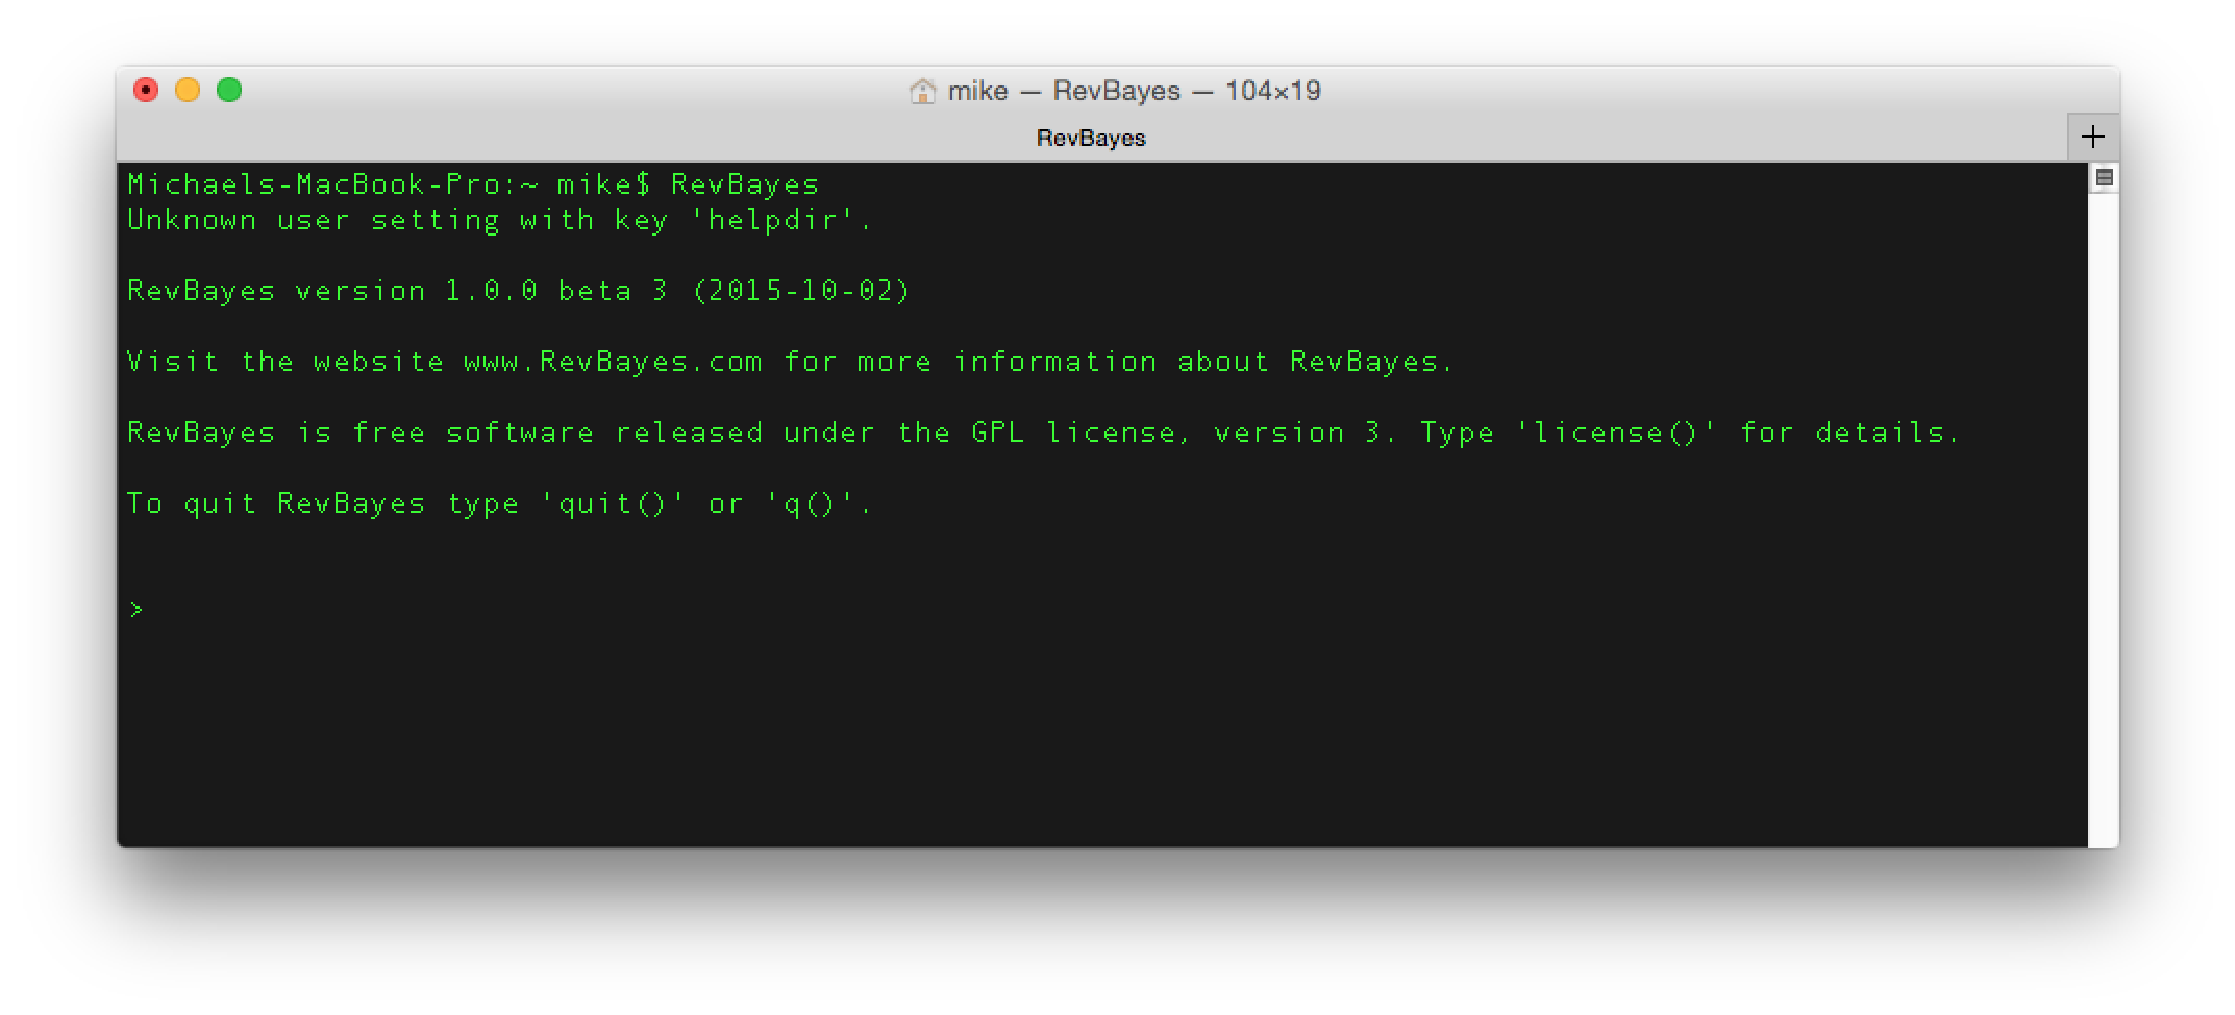
\includegraphics[width=\linewidth]{figures/terminal.pdf}
\end{figure}

\subsection{Operators and Functions}

\Rev is an interpreted language for statistical computing and phylogenetic analysis.
Therefore, the basics are simple mathematical operations.
Entering each of the following lines will automatically execute these operations.
{\tt \begin{snugshade*}
\begin{lstlisting}    
# Simple mathematical operators:
1 + 1                            # Addition
10 - 5                           # Subtraction
5 * 5                            # Multiplication
10 / 2                           # Division
2^3                              # Exponentiation
5%2                              # Modulo
\end{lstlisting}
\end{snugshade*}}

\begin{figure}[H]
	\centering
	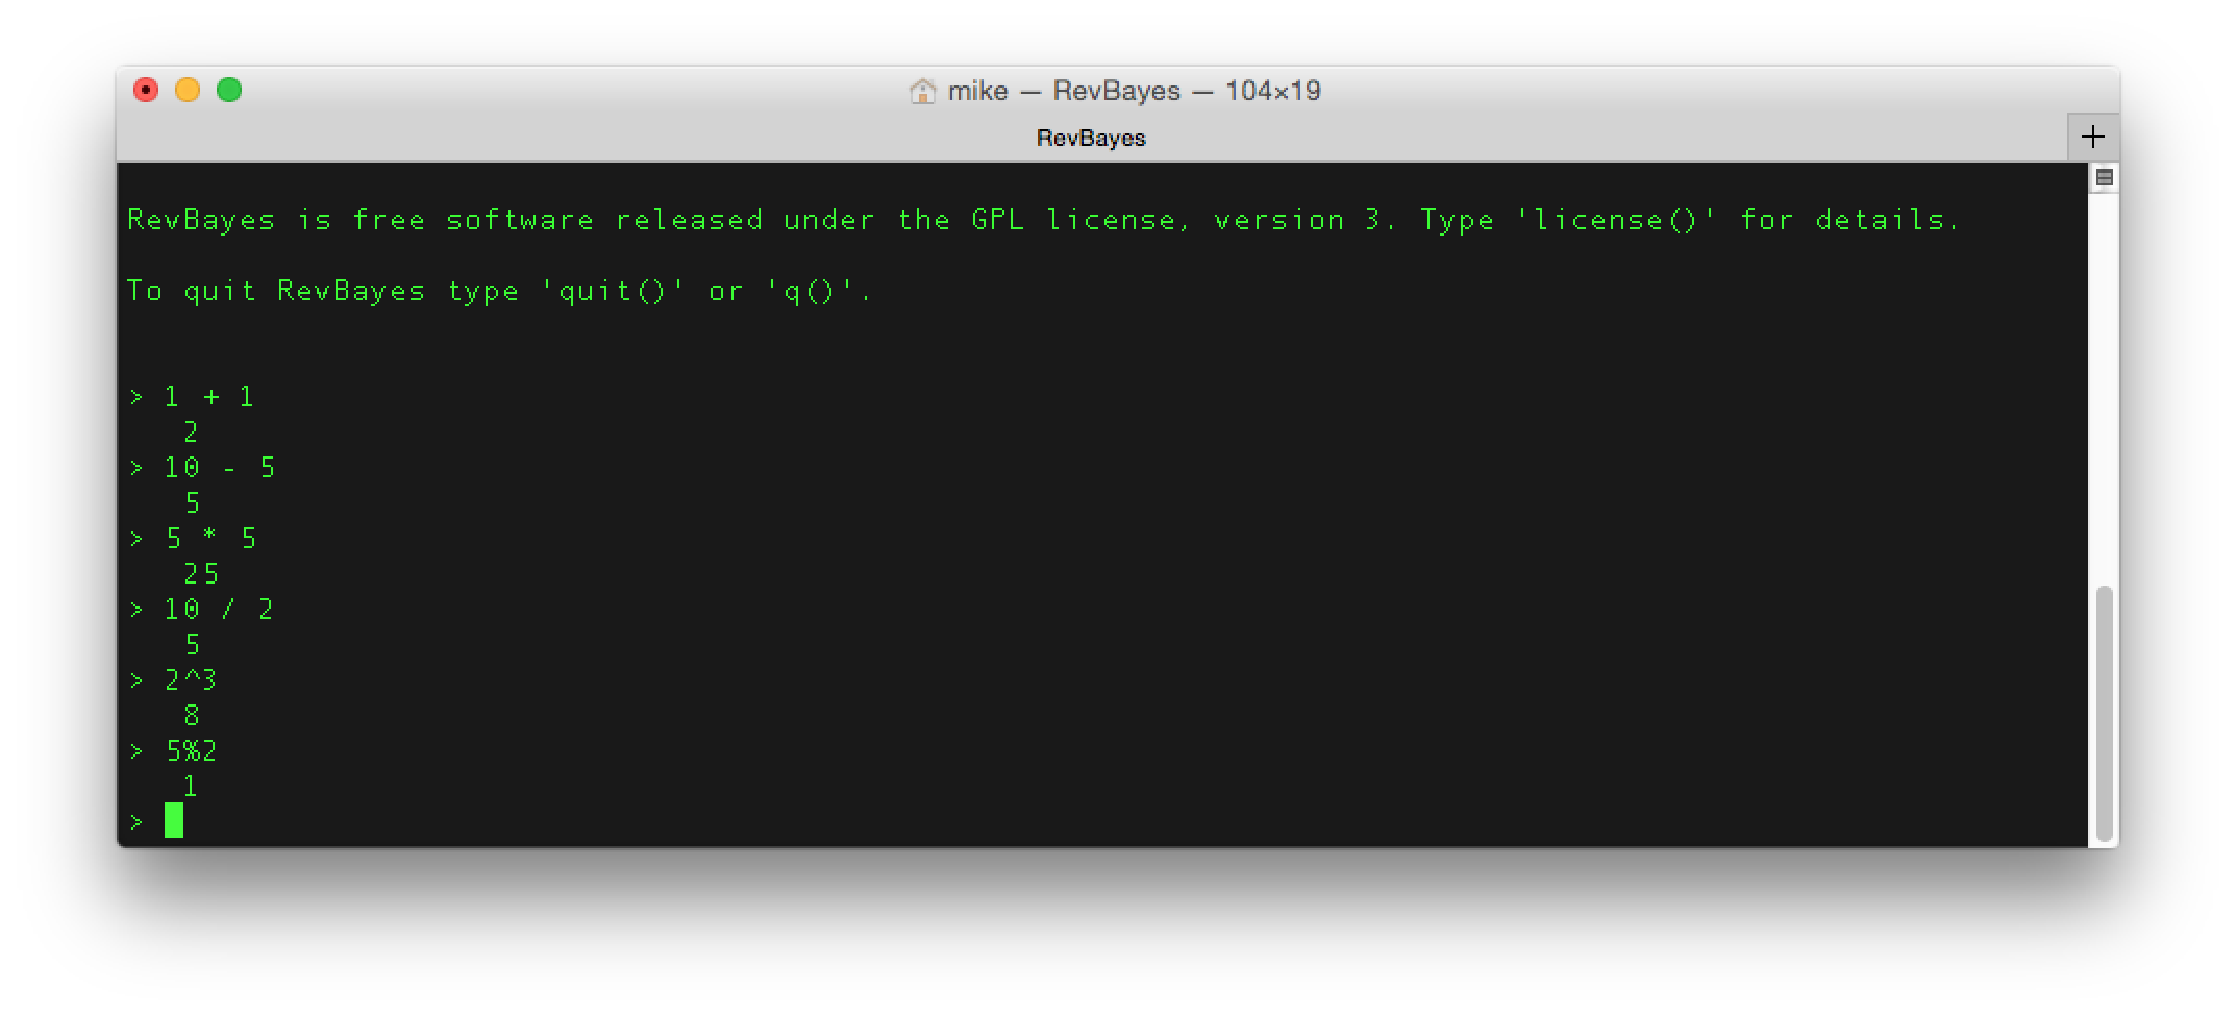
\includegraphics[width=\linewidth]{figures/revbayes_operations.pdf}
\end{figure}
\noindent From now on, we will omit images of the terminal.

Each set of operations constitutes a \emph{statement}.
As you work through these tutorials, it is helpful to write the statements you enter into a blank text file, then copy-and-paste the statements into \Rev to execute them.
This way, you have a complete history of everything you've done, and can easily start over without having to rewrite everything.
We refer to the text file containing the list of commands as a \emph{script}, because it describes line-by-line instructions for the program to follow.

You can write multiple statements in the same line if you separate them by a semicolon (\texttt{;}).
The statements will execute as if you wrote each on a single line.
{\tt \begin{snugshade*}
\begin{lstlisting}    
1 + 1; 2 + 2                    # Multiple statements in one line
\end{lstlisting}
\end{snugshade*}}

Here you can see that comments always start with the hash symbol (\texttt{\#}).
Everything after the `\texttt{\#}'-symbol will be ignored.
In addition to these simple mathematical operations, \Rev provides some standard math functions which can be called by:
{\tt \begin{snugshade*}
\begin{lstlisting}    
# Math functions
exp(1)                           # exponential function
ln(1)                            # logarithmic function with natural base
sqrt(16)                         # square root function 
power(2,2)                       # power function: power(a,b) = a^b
\end{lstlisting}
\end{snugshade*}}
Notice that \Rev is case-sensitive.
That means, \Rev distinguishes upper and lower case letter for both variable names and function names.
For example, only the first of these two calls will work:
{\tt \begin{snugshade*}
\begin{lstlisting}    
exp(1)                           # correct lower case name
Exp(1)                           # wrong upper case name
\end{lstlisting}
\end{snugshade*}}

%\clearpage
\subsection{Variable Declaration and Assignment}
One of the most important features of \RevBayes (or any programming language, really) is the ability to declare and assign variables.
Variables store information to be referenced later, and can change throughout the execution of the program.
There are three kinds of variables in \RevBayes, called \emph{constant}, \emph{deterministic}, and \emph{stochastic} variables.
Constant variables contain values that are not random in your model.
Deterministic variables are functions of other variables.
Stochastic variables are random variables in your model, and will change during your analysis; importantly, stochastic variables (being random variables) are always associated with a particular statistical distribution.

Different types of variables differ in how you create them and assign values to them.
We will begin by creating a constant variable with name \texttt{a} that starts with the value 1. 
The left arrow assignment (\texttt{<-}) always creates a constant variable, and automatically assigns the following value to it.
{\tt \begin{snugshade*}
\begin{lstlisting}    
# Variable assignment: constant
a <- 1                           # assignment of constant node `a'
\end{lstlisting}
\end{snugshade*}}
You see the value of `a' by just typing in the variable name and pressing enter.
{\tt \begin{snugshade*}
\begin{lstlisting}    
a                                # printing the value of `a'
\end{lstlisting}
\end{snugshade*}}

Next, we create a deterministic variable \texttt{b} using the \texttt{:=} assignment computed by \texttt{exp(a)} and another deterministic variable \texttt{c} computed by \texttt{ln(b)}. 
Deterministic variables are always created using the colon-equal assignment (\texttt{:=}). 

{\tt \begin{snugshade*}
\begin{lstlisting}    
# Variable assignment: deterministic

# assignment of deterministic node `b' with
# the exponential function with parameter `a'
b := exp(a)  
b

# assignment of deterministic node `c' with
# logarithmic function with parameter `b'
c := ln(b)              
c 
\end{lstlisting}
\end{snugshade*}}

Finally, we will create the third type of variables in \Rev: stochastic variables.
We will create a random variable \texttt{x} from an exponential distribution with parameter \texttt{lambda}.  
Stochastic assignments use the $\sim$ operation.
{\tt \begin{snugshade*}
\begin{lstlisting}     
# Variable assignment: stochastic

# assign constant node `lambda' with value `1'
lambda <- 1.0

# create stochastic node with exponential 
# distribution and parameter `lambda'
x ~ dnExponential(lambda)
\end{lstlisting}
\end{snugshade*}}
The value of \texttt{x} is a random draw from the distribution. 
You can see the value and the probability (or log-probability) of the current value under the current parameter values by
{\tt \begin{snugshade*}
\begin{lstlisting}    
x                                # print value of stochastic node `x'
x.probability()                  # print the probability if `x'
x.lnProbability()                # print the log-probability if `x'
\end{lstlisting}
\end{snugshade*}}



\subsection{Distributions and Random Numbers}

\Rev provides functions for common statistical distributions.
We'll demonstrate by generating random exponential numbers as we did in lecture.
Recall that we can transform a random variable $u$ sampled from a Uniform(0,1) distribution into an exponential distribution with rate parameter $\lambda$:
\begin{align*}
	u &\sim \text{Uniform(0,1)}\\
	x &= -\frac{1}{\lambda \ln u}
\end{align*}
In \Rev, we might describe $u$ as a stochastic variable, and $x$ as a deterministic variable (since it is a function of $u$):
{\tt \begin{snugshade*}
\begin{lstlisting}
# create the random variable u
u ~ dnUniform(0,1)
u

# determine the rate parameter
lambda <- 1.0

# create x as a deterministic function of u
x := - 1 / lambda * ln(u)
x
\end{lstlisting}
\end{snugshade*}}
\noindent Alternatively, we can create $x$ directly as an exponential random variable:
{\tt \begin{snugshade*}
\begin{lstlisting}
# create the random variable x
x ~ dnExponential(lambda)
x
\end{lstlisting}
\end{snugshade*}}



\subsection{Vectors}
Individual variables can have more than one value.
Variables that have more than one value are called \emph{vectors}.
The simplest way to create a vector is like this:
{\tt \begin{snugshade*}
\begin{lstlisting}    
v <- v(1.0,2.0,3.0)              # create a vector
\end{lstlisting}
\end{snugshade*}}
\noindent You can refer to a specific value in the vector using brackets, \texttt{[i]}, where \texttt{i} is the index of the variable of interest.
{\tt \begin{snugshade*}
\begin{lstlisting}    
v[1]                             # print the first entry
v[1] <- 10                       # change the value of the first entry
v
\end{lstlisting}
\end{snugshade*}}



\subsection{\texttt{for} loops}
\texttt{for} loops are important programming structures that allow you to repeat the same statement a number of times on different variables.
The basic structure of a \texttt{for} loop is:
{\tt \begin{snugshade*}
\begin{lstlisting}    
# a for loop
for (<variable> in <set of values>) {
   <statements using variable>
}
\end{lstlisting}
\end{snugshade*}}
\noindent The \texttt{for} statement is followed by a set of parenthesis containing \texttt{<variable>}, which contains the name of the variable being iterated, and \texttt{<set of values>}, which are the values that the variable iterates over.
The \texttt{for} loop variable is a special variable that is created by the \texttt{for} loop: you do not have to create it before executing the loop.
This simple \texttt{for} loop creates the variable \texttt{i}, and for each value of \texttt{i} from 1 to 100, prints the value of \texttt{i} to the screen.
{\tt \begin{snugshade*}
\begin{lstlisting}    
for (i in 1:100) {
  i
}
\end{lstlisting}
\end{snugshade*}}

\noindent \texttt{for} loops are very powerful programming tools.
We can use a \texttt{for} loop to create an entire \emph{vector} of uniform random numbers, and transform them into a \emph{second} vector of exponential random numbers.
{\tt \begin{snugshade*}
\begin{lstlisting}    
for (i in 1:100) {
  u[i] ~ dnUniform(0,1)
  x[i] := - 1.0 / lambda * ln(u[i])
}
\end{lstlisting}
\end{snugshade*}}

\noindent Close \Rev using the statement \texttt{q()}.
{\tt \begin{snugshade*}
\begin{lstlisting}    
q()
\end{lstlisting}
\end{snugshade*}}

\subsection{References}

\bibliographystyle{sysbio}
\bibliography{\GlobalResourcePath refs}
